% Generated by Listas/make_statements.py from pratica-lecture-08.md, item 4. Do not edit.
\textbf{Source.} Muñoz-Garcia \& Toro-Gonzalez (2019), \emph{Strategy and Game Theory: Practice Exercises with Answers}, Ch. 9, Exercise 1 ``Finding Separating and Pooling Equilibria'', pp.~376--377 {[}PDF pp.~385--386{]}. Reproduced verbatim (statement only; the book's worked answer follows it). Answer: yes, the book's worked answer follows the exercise.



\begin{quote}

Consider the following game of incomplete information: nature first determines player 1's type, either high or low, with equal probabilities. Then player 1, observing his own type, decides whether to choose left (L) or Right (R). If he chooses left, the game ends and players' payoffs become \((u_1, u_2) = (2, 0)\), regardless of player 1's type. Figure 9.1 depicts these payoffs in the left-hand side of the tree. If, instead, player 1 chooses Right, player 2 is called on to move. In particular, without observing whether player 1's type is high or low, player 2 must respond by either selecting Up (U) or Down (D). As indicated by the payoffs in the right-hand side of the tree, when player 1's type is high, player 2 prefers to play Up. The opposite preference ranking applies when player 1's type is low.



\pandocbounded{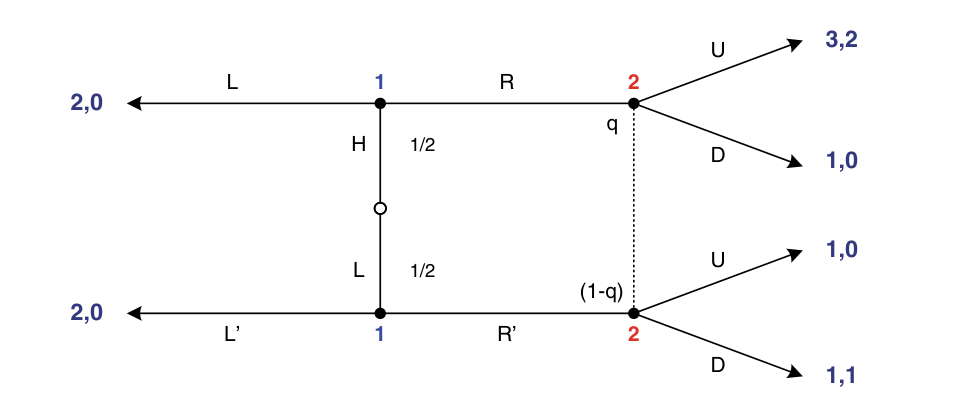
\includegraphics[keepaspectratio,alt={Fig. 9.1 Game tree where player 2 is uninformed}]{../figures/munoz-garcia-9-1.png}}



\emph{Fig. 9.1} Game tree where player 2 is uninformed



\textbf{Part (a)} Does this game have a Separating Perfect Bayesian Equilibrium (PBE)?



\textbf{Part (b)} Does this game have a Pooling PBE?

\end{quote}

